\documentclass[12pt,aspectratio=169]{beamer}

\usetheme{CSCS}

\graphicspath{{./figs/}}

% define footer text
\newcommand{\footlinetext}{CSCS-USI Summer School 2018}

% Select the image for the title page
\newcommand{\picturetitle}{cscs_images/cscs_entrance_painting.pdf}

\lstdefinestyle{shstyle}{
  basicstyle=\scriptsize\ttfamily,
  keywordstyle=\color{blue},
  stringstyle=\color{magenta},
  commentstyle=\itshape\color{cscsred},
  language=bash,
}

\newcommand\shinline[2][]{\lstinline[style=shstyle,basicstyle=\ttfamily,#1]!#2!}

% Please use the predifined colors:
% cscsred, cscsgrey, cscsgreen, cscsblue, cscsbrown, cscspurple, cscsyellow,
% cscsblack, cscswhite

\author{\emph{Vasileios Karakasis, CSCS}}
\title{GPU programming using OpenACC}
\subtitle{CSCS-USI Summer School 2018}
\date{July 18--19, 2018}

\begin{document}

% TITLE SLIDE
\cscstitle

\begin{frame}{Goals of the course}
  \begin{itemize}
  \item Part I
    \begin{itemize}
    \item Basic concepts
      \begin{itemize}
      \item Execution and memory model
      \item Basic directives
      \item Profiling and debugging
      \item Hands-on sessions
      \end{itemize}
    \item Advanced topics
      \begin{itemize}
      \item Asynchronous execution and wait queues
      \item Interoperability with CUDA and MPI
      \item Deep copy
      \item Hands-on sessions
      \end{itemize}
    \end{itemize}
  \item  Part II
    \begin{itemize}
    \item Port the miniapp to GPU using OpenACC
    \item Walk away ready to start hacking your own code
    \end{itemize}
  \end{itemize}
\end{frame}

%% \begin{frame}{Overview}
%%   \begin{itemize}
%%   \item Day 1 (Understand the basic concepts of OpenACC)
%%     \begin{itemize}
%%     \item Execution and memory model
%%     \item Basic directives
%%     \item Profiling and debugging
%%     \item Hands-on sessions
%%     \end{itemize}
%%     \vspace\baselineskip
%%   \item Day 2 (Advanced topics)
%%     \begin{itemize}
%%     \item Asynchronous execution and wait queues
%%     \item Interoperability with CUDA and MPI
%%     \item Deep copy
%%     \item Hands-on sessions
%%     \end{itemize}
%%   \end{itemize}
%% \end{frame}

\begin{frame}{What is OpenACC?}
  \begin{itemize}
  \item Collection of compiler directives for specifying loops and regions to be
    offloaded from a host CPU to an attached accelerator device
  \item Host + Accelerator programming model
  \item High-level representation
  \item Current specification version: 2.6
  \end{itemize}
\end{frame}

\begin{frame}{Why to use OpenACC?}
  Because \dots
  \vspace\baselineskip
  \begin{itemize}
  \item I don't care about all the little hardware details, I want my science done.
  \item I want to run on accelerators, but I still need a fast and readable code.
  \item I need portability across different accelerator vendors, but also be able to run on the multicore.
  \item I inhereted a large legacy monolithic codebase, which I don't dare to
    refactor completely, but I need to get my results faster.
  \item My code is in Fortran.
  \end{itemize}
\end{frame}

\begin{frame}{OpenACC is not a silver bullet}
  \begin{itemize}
  \item A high-level representation is not a panacea.
    \begin{itemize}
    \item You still need to understand and adapt to the programming model.
    \end{itemize}
    \vfill
  %% \item Be ware of avoiding a \lstinlineCpp{\#pragma}-clutter
  %%   \begin{itemize}
  %%   \item Rethink and refactor
  %%   \end{itemize}
  \item Does not substitute hand-tuning, but can serve as a very good starting point.
    \begin{itemize}
    \item Some low-level CUDA constructs are not exposed (shared memory, groups etc.)
    \end{itemize}
    \vfill
  \item User base not yet as large as of classic OpenMP for multicores, but it is expanding.
    \begin{itemize}
    \item You may run into compiler bugs or specification ambiguities.
    \end{itemize}
  \end{itemize}
\end{frame}

\begin{frame}[fragile]{Format of directives}
  \begin{itemize}
  \item C/C++
    \begin{itemize}
    \item \lstinlineCpp{\#pragma acc} \emph{directive-name [clause-list]
      new-line}
    \item Scope is the following \emph{block of code}
    \end{itemize}
  \item Fortran
    \begin{itemize}
    \item \lstinlineFortran{\!\$acc} \emph{directive-name [clause-list]
      new-line}
    \item Scope is until \lstinlineFortran{\!\$acc end} \emph{directive-name}
    \end{itemize}
  \end{itemize}
\end{frame}

\begin{frame}{Programming model}
  \begin{itemize}
  \item Host-directed execution
  \item Compute intensive regions are offloaded to attached accelerator devices
  \item Host orchestrates the execution on the device
    \begin{itemize}
    \item Allocations on the device
    \item Data transfers
    \item Kernel launches
    \item Wait for events
    \item Etc\dots
    \end{itemize}
  \end{itemize}
\end{frame}

\begin{frame}{Execution model}
  \begin{itemize}
  \item The device executes \emph{parallel} or \emph{kernel regions}
  \item Parallel region
    \begin{itemize}
    \item Work-sharing loops
    \end{itemize}
  \item Kernel region
    \begin{itemize}
    \item Multiple loops to be executed as multiple kernels
    \end{itemize}
  \item Levels of parallelim
    \begin{enumerate}
    \item \emph{Gang} \onslide<2->{\emph{$\rightarrow$ CUDA block}}
    \item \emph{Worker} \onslide<2->{\emph{$\rightarrow$ CUDA warp}}
    \item \emph{Vector} \onslide<2->{\emph{$\rightarrow$ CUDA threads}}
    \end{enumerate}
    \begin{itemize}
    \item Parallelism levels are decided by the compiler but can be fine-tuned by
      the user
    \onslide<2->{
      {\color{cscsred} \item Mapping to CUDA blocks/warps/threads is implementation defined}
    }
    \end{itemize}
  \end{itemize}
\end{frame}

\begin{frame}{Execution model}{Modes of execution}
  \begin{itemize}
  \item Gang
    \begin{itemize}
    \item Gang-redundant (GR)
    \item Gang-partioned (GP)
    \end{itemize}
  \item Worker
    \begin{itemize}
    \item Worker-single (WS)
    \item Worker-partitioned (WP)
    \end{itemize}
  \item Vector
    \begin{itemize}
    \item Vector-single (VS)
    \item Vector-partitioned (VP)
    \end{itemize}
  \end{itemize}
\end{frame}

\begin{frame}{Execution model}{Modes of execution}
  \begin{figure}
    \centering
    \only<1>{
      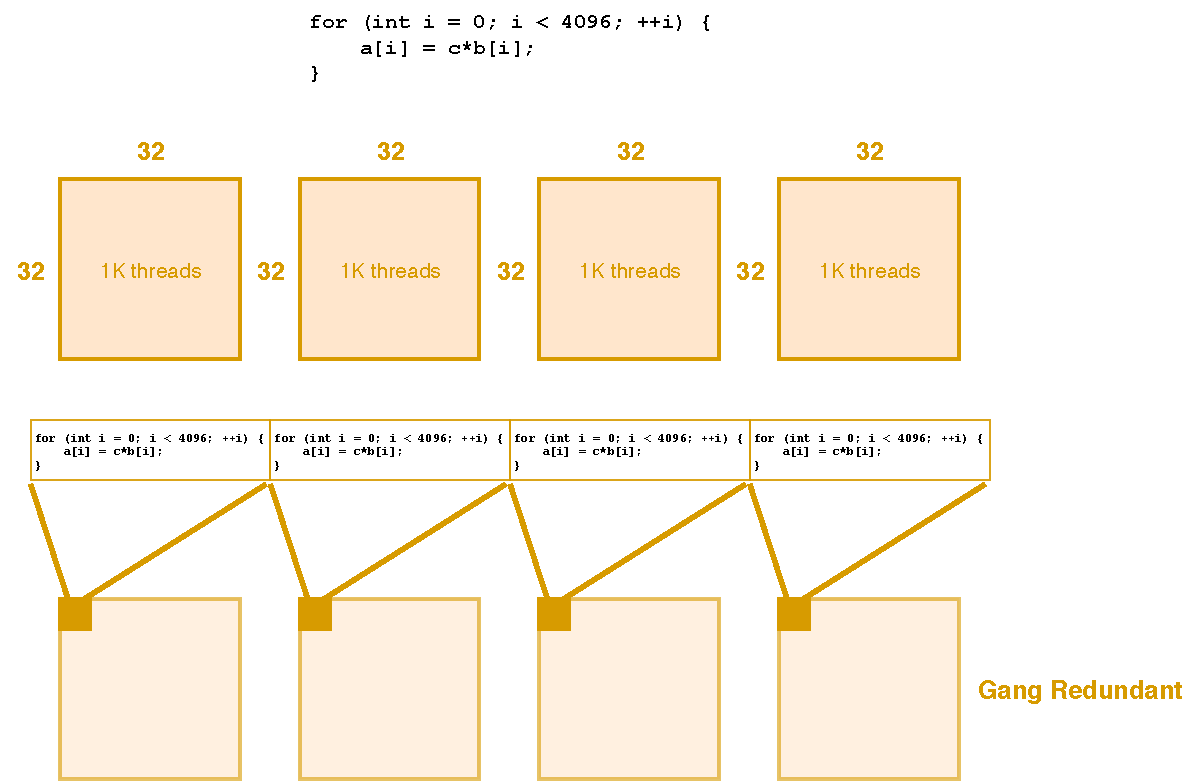
\includegraphics[height=.8\textheight]{GR_mode}
    }
    \only<2>{
      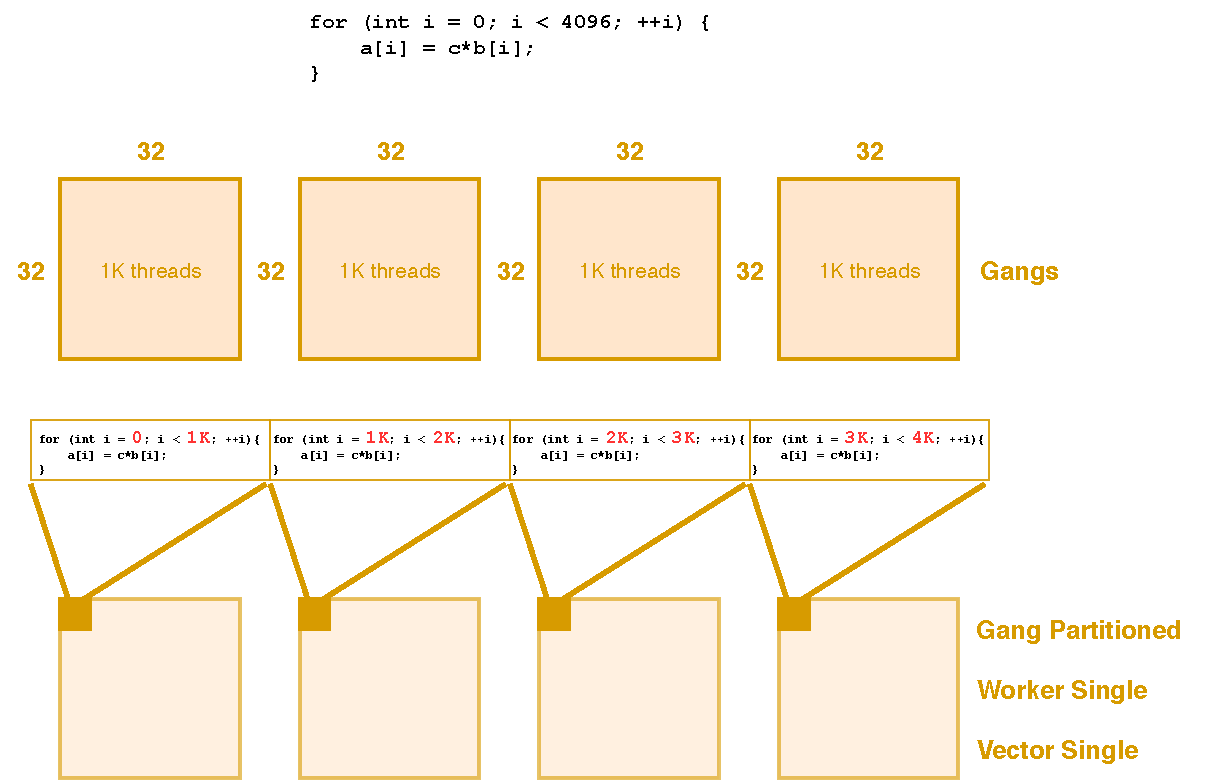
\includegraphics[height=.8\textheight]{GP_WS_VS_mode}
    }
    \only<3>{
      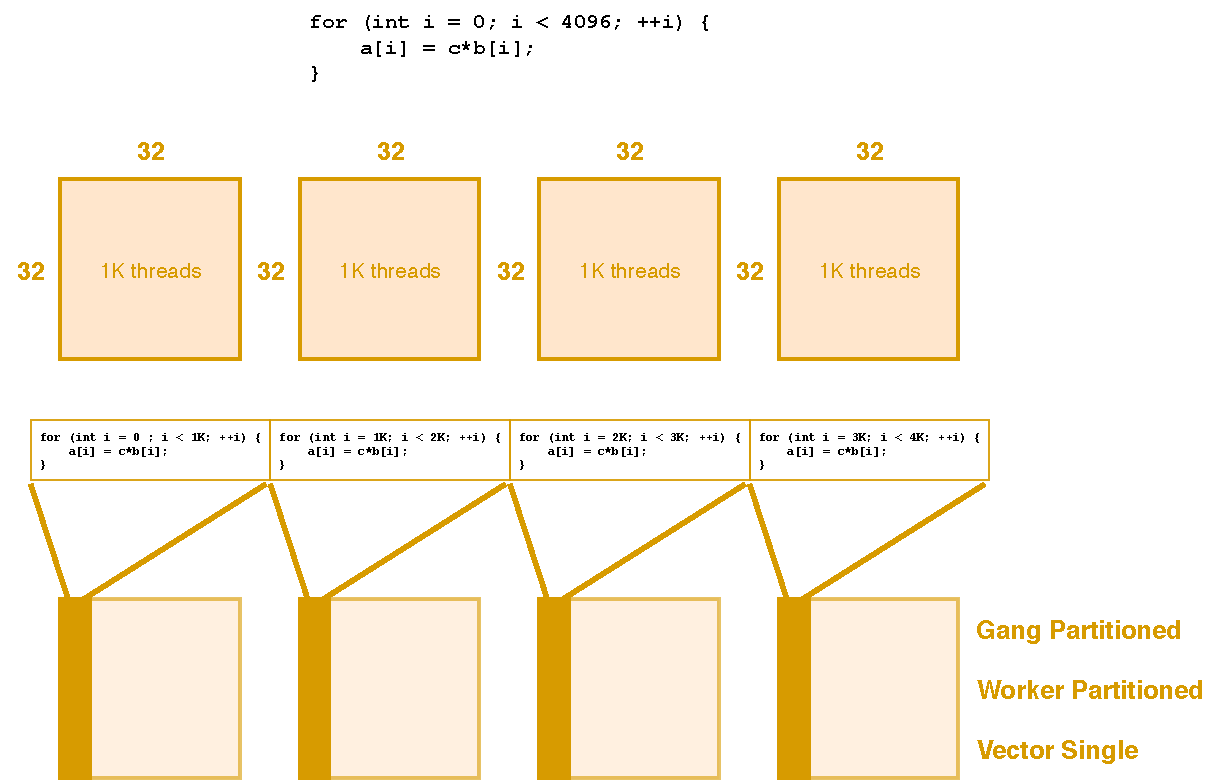
\includegraphics[height=.8\textheight]{GP_WP_VS_mode}
    }
    \only<4>{
      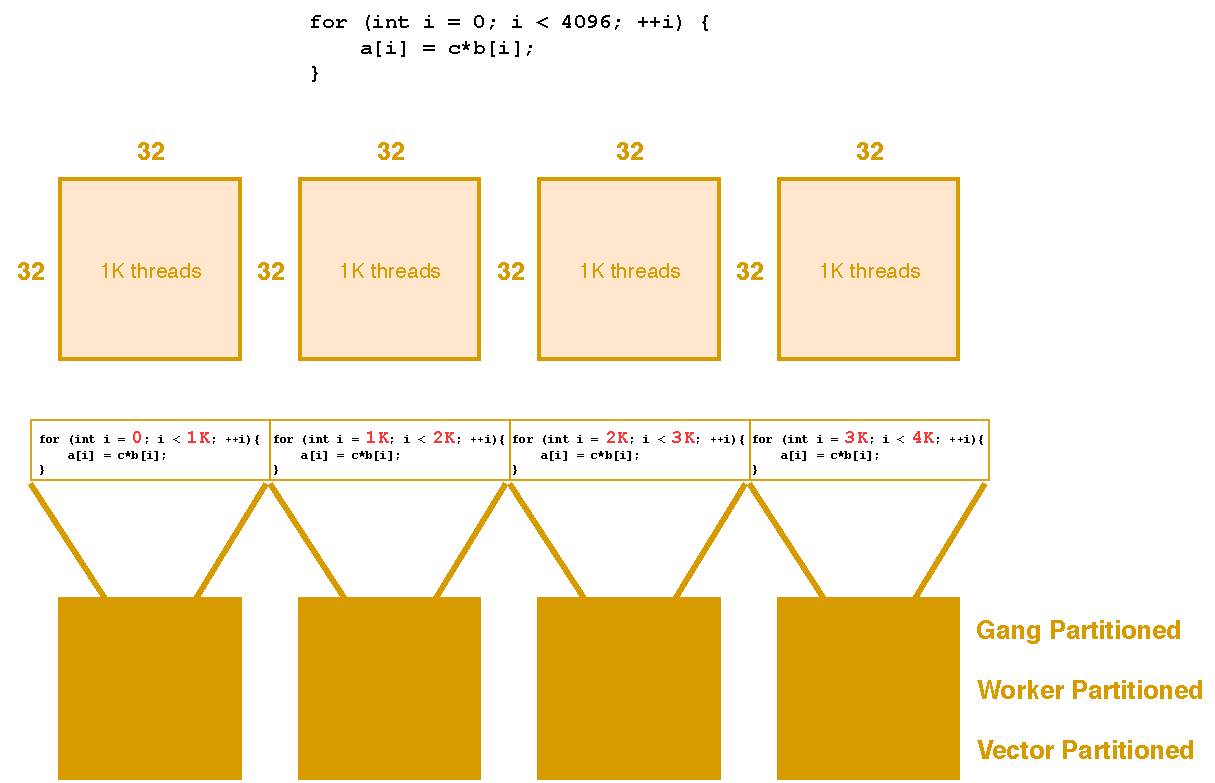
\includegraphics[height=.8\textheight]{GP_WP_VP_mode}
    }
  \end{figure}
\end{frame}


\begin{frame}[fragile]{Execution model}{The \lstinlineCpp{kernels} construct}
  \begin{Fortranlisting}{Multiple loops inside kernels construct}
!$acc kernels
    !GR mode
    do i = 1, N
        !compiler decides on the partitioning (GP/WP/VP modes)
        y(i) = y(i) + a*x(i)
    enddo
    do i = 1, N
        !compiler decides on the partitioning (GP/WP/VP modes)
        y(i) = b*y(i) + a*x(i)
    enddo
!$acc end kernels
  \end{Fortranlisting}
  \begin{itemize}
  \item Compiler will try to deduce parallelism
  \item Loops are launched as different GPU kernels
  \end{itemize}
\end{frame}

\begin{frame}[fragile]{Execution model}{The \lstinlineCpp{parallel} construct}
  \begin{Fortranlisting}{Parallel construct}
!$acc parallel
    do i = 1, N
        ! loop executed in GR mode
        y(i) = y(i) + a*x(i)
    enddo
    !$acc loop
    do i = 1, N
        !compiler decides on the partitioning (GP/WP/VP modes)
        y(i) = b*y(i) + a*x(i)
    enddo
!$acc end parallel
  \end{Fortranlisting}
  \begin{itemize}
  \item No automatic parallelism deduction $\rightarrow$ parallel loops must
    be specified explicitly
  \item Implicit gang barrier at the end of \lstinlineCpp{parallel}
  \end{itemize}
\end{frame}

\begin{frame}{Execution model}{Work-sharing loops}
  \begin{itemize}
  \item C/C++: \lstinlineCpp{\#pragma acc loop}
    \begin{itemize}
    \item Applies to the immediately following \lstinlineCpp{for} loop
    \end{itemize}
  \item Fortran: \lstinlineFortran{\!\$acc loop}
    \begin{itemize}
    \item Applies to the immediately following \lstinlineCpp{do} loop
    \end{itemize}
  \item Loop will be automatically striped and assigned to different threads
    \begin{itemize}
    \item Use the \lstinlineCpp{independent} clause to force striping
    \end{itemize}
  \item Convenience syntax combines
    \lstinlineCpp{parallel}/\lstinlineCpp{kernels} and \lstinlineCpp{loop}
    constructs
    \begin{itemize}
    \item \lstinlineCpp{\#pragma acc parallel loop}
    \item \lstinlineCpp{\#pragma acc kernels loop}
    \item \lstinlineFortran{\!\$acc parallel loop}
    \item \lstinlineFortran{\!\$acc kernels loop}
    \end{itemize}
  \end{itemize}
\end{frame}

\begin{frame}[fragile]{Execution model}{Work-sharing loops -- the \lstinlineCpp{collapse} clause}
  \begin{Fortranlisting}{Collapse loops}
!$acc loop collapse(2)
do i = 1,N
    do j = 1,N
        A(i,j) = coeff*B(i,j)
    enddo
enddo
  \end{Fortranlisting}
  \begin{itemize}
  \item OpenACC vs.\ OpenMP
    \begin{itemize}
    \item OpenACC: apply the \lstinlineCpp{loop} directive to the following $N$
      loops and possibly collapse their iteration spaces if independent
    \item OpenMP: Collapse the iteration spaces of the following $N$ loops
    \end{itemize}
  \end{itemize}
\end{frame}

\begin{frame}[fragile]{Execution model}{Controlling parallelism}
  \begin{itemize}
  \item Amount of parallelism at the \lstinlineCpp{kernels} and
    \lstinlineCpp{parallel} level
    \begin{itemize}
    \item \lstinlineCpp{num_gangs(...)}, \lstinlineCpp{num_workers(...)},
      \lstinlineCpp{vector_length(...)}
    \end{itemize}
  \item At the \lstinlineCpp{loop} level
    \begin{itemize}
    \item \lstinlineCpp{gang}, \lstinlineCpp{worker}, \lstinlineCpp{vector}
    \end{itemize}
  \end{itemize}

  \begin{Fortranlisting}{100 thread blocks with 128 threads each}
!$acc parallel num_gangs(100), vector_length(128)
    !$acc loop gang, vector
    do i = 1, n
        y(i) = y(i) + a*x(i)
    enddo
!$acc end parallel
  \end{Fortranlisting}
\end{frame}

\begin{frame}[fragile]{Execution model}{Variable scoping}
  \begin{itemize}
  \item Allowed in the \lstinlineCpp{parallel} directive only
  \item By default, if outside of a code block, variables are shared in global memory
  \item \lstinlineCpp{private}: A copy of the variable is placed in each \emph{gang} (CUDA block)
  \item \lstinlineCpp{firstprivate}: Same as \lstinlineCpp{private} but initialized from the host value
  \end{itemize}
  \pause
  Implicit scoping:
  \begin{itemize}
  \item (C/C++/Fortran) Loop variables are private to the \emph{thread} that executes the loop
  \item (C/C++ only) Scope of variables declared inside a parallel block depends on the current execution mode:
    \begin{itemize}
    \item \emph{Vector-partitioned} mode $\rightarrow$ private to the thread
    \item \emph{Worker-partitioned, Vector-single} mode $\rightarrow$ private to the worker
    \item \emph{Worker-single} mode $\rightarrow$ private to the gang
    \end{itemize}
  \end{itemize}
\end{frame}

\begin{frame}[fragile]{Execution model}{Reduction operations}
  \begin{itemize}
  \item \lstinlineCpp{\#pragma acc parallel reduction(<op>:<var>)}
    \begin{itemize}
    \item e.g., \lstinlineCpp{\#pragma acc parallel reduction(+:sum)}
    \end{itemize}
  \item \lstinlineCpp{\#pragma acc loop reduction(<op>:<var>)}
  \item \lstinlineCpp{var} must be scalar
  \item \lstinlineCpp{var} is copied and default initialized within each gang
  \item Intermediate results from each gang are combined and made available outside the parallel region
  \item Complex numbers are also supported
  \item Operators: \lstinlineCpp{+}, \lstinlineCpp{*}, \lstinlineCpp{max}, \lstinlineCpp{min}, \lstinlineCpp{&}, \lstinlineCpp{|}, \lstinlineCpp{\%}, \lstinlineCpp{&&}, \lstinlineCpp{||}
  \end{itemize}
\end{frame}

\begin{frame}[fragile]{Execution model}{Calling functions from parallel regions}
  \begin{itemize}
  \item \lstinlineCpp{\#pragma acc routine \{gang | worker | vector | seq\}}
    \begin{itemize}
    \item Just before the function declaration or definition
    \end{itemize}
  \item \lstinlineFortran{\!\$acc routine \{gang | worker | vector | seq\}}
    \begin{itemize}
    \item In the specification part of the subroutine
    \end{itemize}
  \item Parallelism level of the routine
    \begin{itemize}
    \item \lstinlineCpp{gang}: must be called from GR context
    \item \lstinlineCpp{worker}: must be called from WS context
    \item \lstinlineCpp{vector}: must be called from VS context
    \item \lstinlineCpp{seq}: must be called from sequential context
    \end{itemize}
  \end{itemize}
\end{frame}

\begin{frame}[fragile]{Memory model}{Where is my data?}
  \begin{itemize}
  \item The host and the device have separate address spaces
    \begin{itemize}
    \item Data management between the host and the device is the programmer's responsibility
    \item You must make sure that all the necessary data for a computation is available on the accelerator before entering the compute region
    \item You must make sure to transfer the processed data back to the host if needed
    \end{itemize}
    \pause
    \vspace\baselineskip
  \item But there can be some exceptions:
    \begin{itemize}
    \item The ``device'' might be the multicore $\rightarrow$ no need for data management
    \item Some compilers may infer automatically the necessary data transfers
    \item Nvidia Pascal GPUs provide efficient support for a unified memory view between the host and the accelerator
    \end{itemize}
  \end{itemize}
\end{frame}

\begin{frame}{Memory model}{Separate address spaces}
  \begin{figure}
    \centering
    \only<1>{
      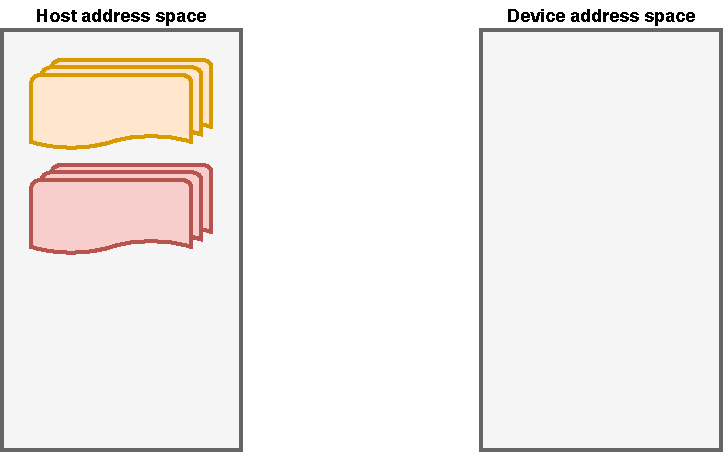
\includegraphics[height=.7\textheight]{mem_model_init}
    }
    \only<2>{
      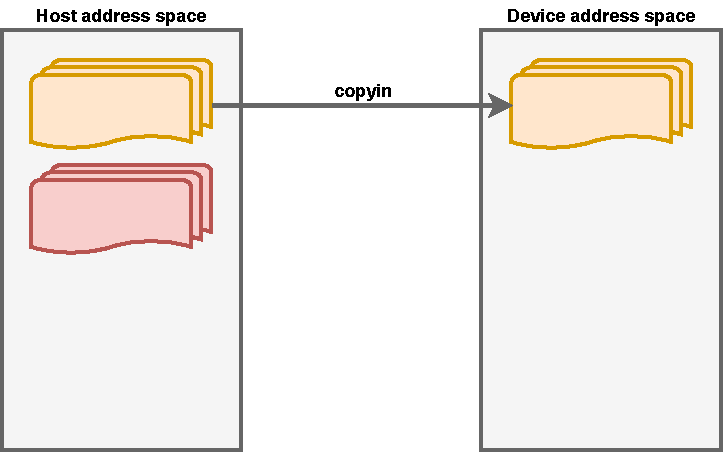
\includegraphics[height=.7\textheight]{mem_model_copyin1}
    }
    \only<3>{
      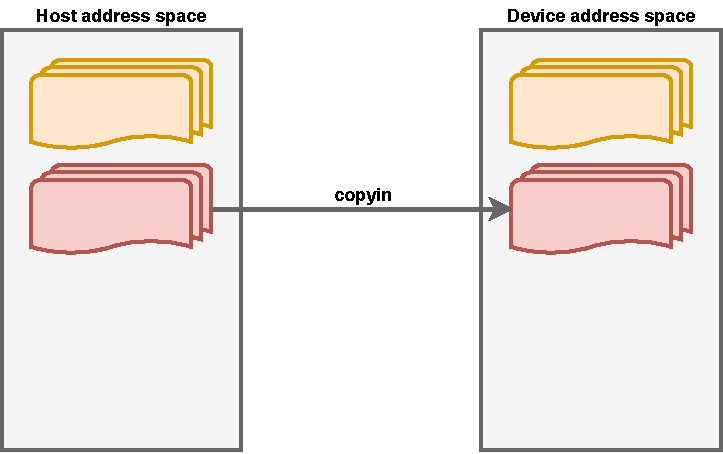
\includegraphics[height=.7\textheight]{mem_model_copyin2}
    }
    \only<4>{
      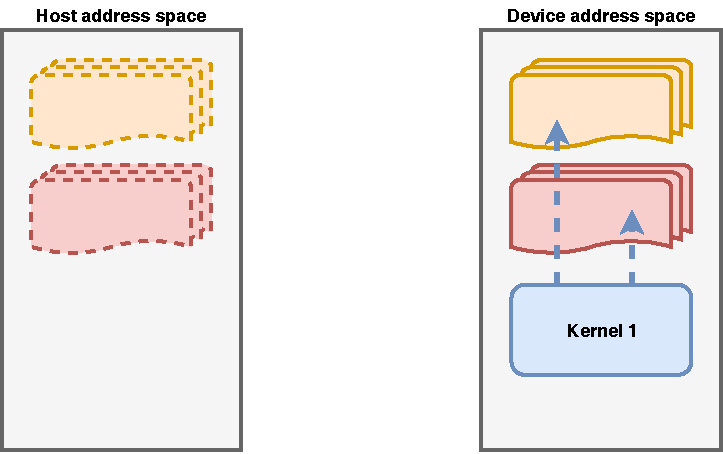
\includegraphics[height=.7\textheight]{mem_model_kernel1}
    }
    \only<5>{
      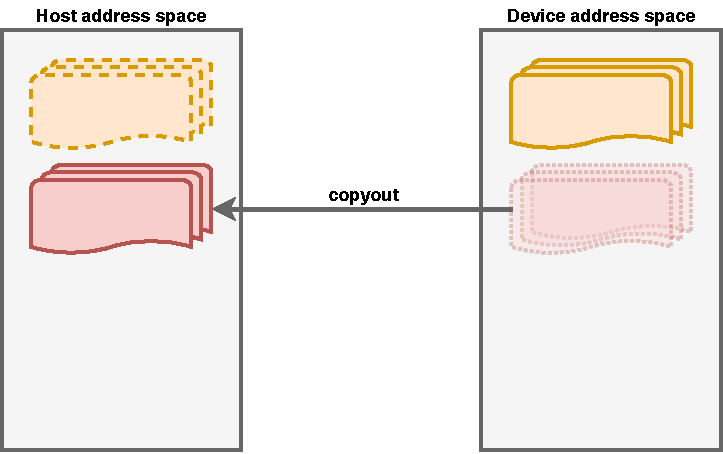
\includegraphics[height=.7\textheight]{mem_model_copyout2}
    }
    \only<6>{
      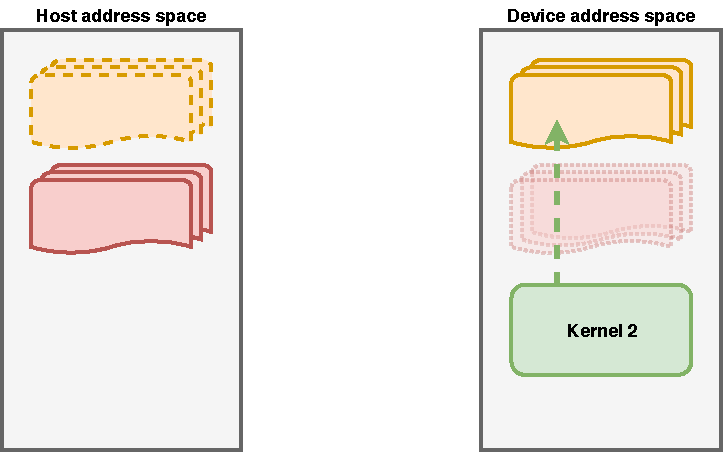
\includegraphics[height=.7\textheight]{mem_model_kernel2}
    }
    \only<7>{
      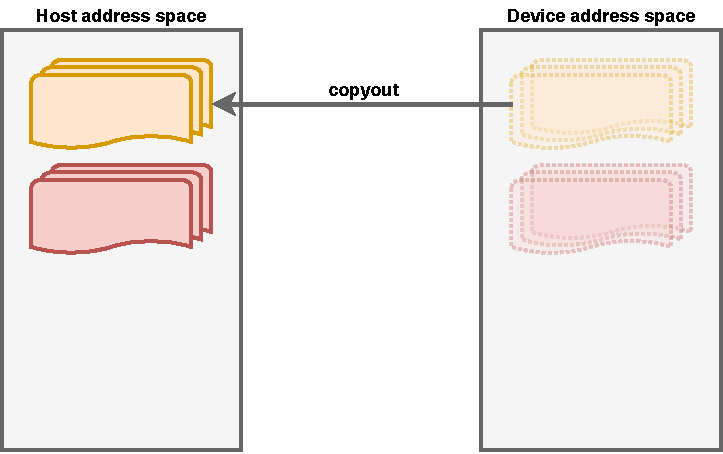
\includegraphics[height=.7\textheight]{mem_model_copyout1}
    }
  \end{figure}
\end{frame}

\begin{frame}{Memory model}{Unified memory address space}
  \begin{figure}
    \centering
    \only<1>{
      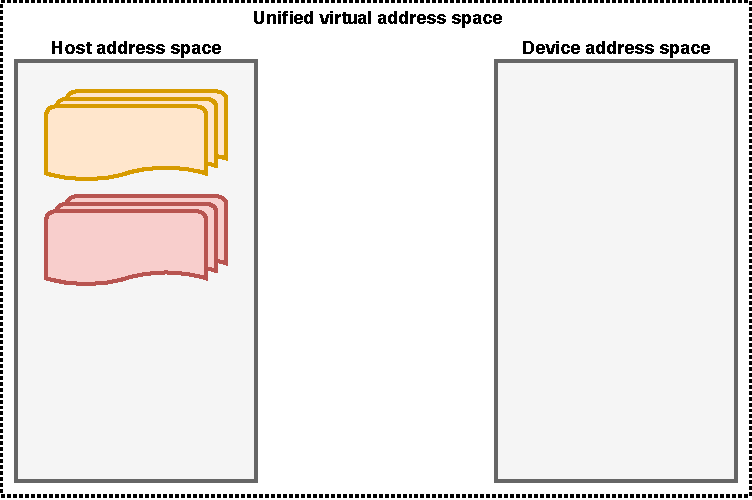
\includegraphics[height=.7\textheight]{unified_mem_init}
    }
    \only<2>{
      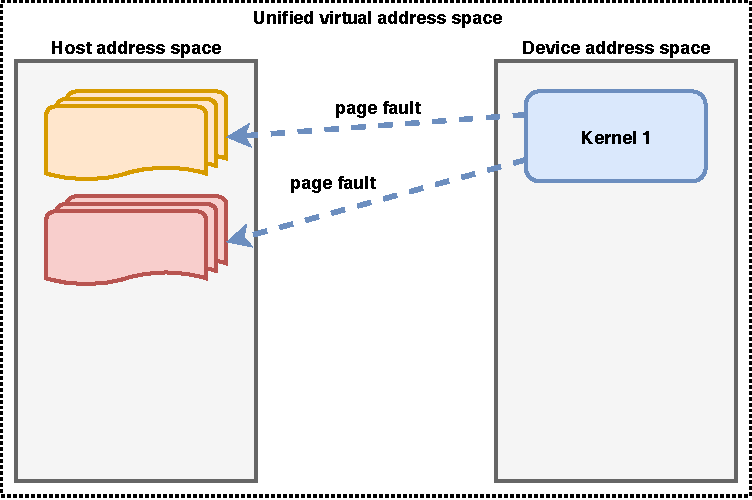
\includegraphics[height=.7\textheight]{unified_mem_pagefault}
    }
    \only<3>{
      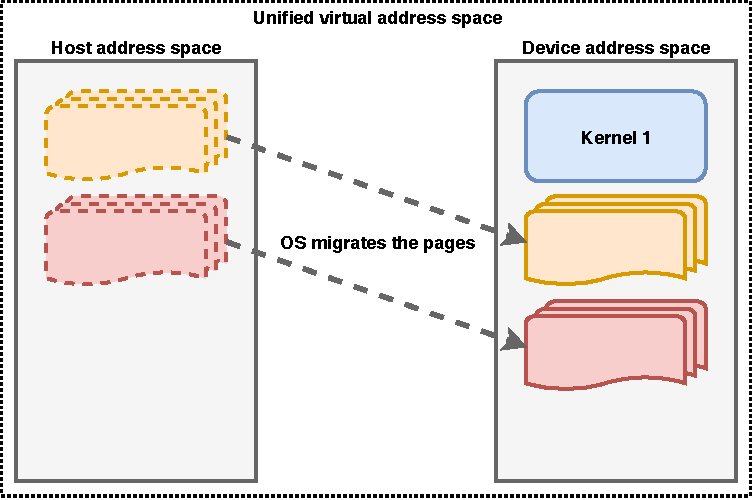
\includegraphics[height=.7\textheight]{unified_mem_pagemigration}
    }
  \end{figure}
\end{frame}

\begin{frame}[fragile]{Memory model}{Directives accepting data clauses}
  Data clauses may appear in the following directives:
    \vspace\baselineskip
  \begin{itemize}
  \item Compute directives:
    \begin{itemize}
    \item\lstinlineCpp{#pragma acc kernels}
    \item\lstinlineCpp{#pragma acc parallel}
    \end{itemize}
    \vspace{.5\baselineskip}
  \item Data directives:
    \begin{itemize}
    \item \lstinlineCpp{#pragma acc data}
    \item \lstinlineCpp{#pragma acc enter data}
    \item \lstinlineCpp{#pragma acc exit data}
    \item \lstinlineCpp{#pragma acc declare}
    \item \lstinlineCpp{#pragma acc update}
    \end{itemize}
  \end{itemize}
\end{frame}

\begin{frame}[fragile]{Memory model}{Data clauses}
  \begin{itemize}
  \item \lstinlineCpp{create(a[0:n])}: Allocate array \lstinlineCpp{a} on device
  \item \lstinlineCpp{copyin(a[0:n])}: Copy array \lstinlineCpp{a} to device
  \item \lstinlineCpp{copyout(a[0:n])}: Copy array \lstinlineCpp{a} from device
  \item \lstinlineCpp{copy(a[0:n])}: Copy array \lstinlineCpp{a} to and from device
  \item \lstinlineCpp{present(a)}: Inform OpenACC runtime that array \lstinlineCpp{a} is on device
  \item \lstinlineCpp{delete(a)}: Deallocate array \lstinlineCpp{a} from device (\lstinlineCpp{exit data} only)
  \end{itemize}
  \vfill
  Not for the \shinline{acc update} directive
\end{frame}

\begin{frame}[fragile]{Memory model}{The \texttt{acc data} directive}
  \begin{itemize}
  \item Defines a scoped data region
    \begin{itemize}
    \item Data will be copied in at entry of the region and copied out at exit
    \item A \emph{structural reference count} is associated with each memory region that appears in the data clauses
    \end{itemize}
    \vfill
  \item C/C++: \lstinlineCpp{#pragma acc data} \emph{\texttt{[data clauses]}}
    \begin{itemize}
    \item The next block of code is a data region
    \end{itemize}
    \vfill
  \item Fortran: \lstinlineFortran{\!\$acc data} \emph{\texttt{[data clauses]}}
    \begin{itemize}
    \item Defines a data region until \lstinlineFortran{\!\$acc end data} is encountered
    \end{itemize}
  \end{itemize}
\end{frame}

\begin{frame}[fragile]{Memory model}{The \texttt{acc enter/exit data} directives}
  \begin{itemize}
  \item Defines an unscoped data region
    \begin{itemize}
    \item Data will be resident on the device until a corresponding \lstinlineCpp{exit data} directive is found
    \item Useful for managing data on the device across compilation units
    \item A \emph{dynamic reference count} is associated with each memory region that appears in the data clauses
    \end{itemize}
    \vfill
  \item C/C++:
    \begin{itemize}
    \item \lstinlineCpp{#pragma acc enter data} \emph{\texttt{[data clauses]}}
    \item\lstinlineCpp{#pragma acc exit data} \emph{\texttt{[data clauses]}}
    \end{itemize}
    \vfill
  \item Fortran:
    \begin{itemize}
    \item \lstinlineFortran{\!\$acc enter data} \emph{\texttt{[data clauses]}}
    \item \lstinlineFortran{\!\$acc exit data} \emph{\texttt{[data clauses]}}
    \end{itemize}
  \end{itemize}
\end{frame}

\begin{frame}[fragile]{Memory model}{The \texttt{acc declare} directive}
  \begin{itemize}
  \item Functions, subroutines and programs define \emph{implicit data regions}
  \item The \lstinlineCpp{acc declare} directive is used in variable declarations for making them available on the device during the lifetime of the implicit data region
  \item Useful for copying global variables to the device
    \vfill
  \item C/C++: \lstinlineCpp{#pragma acc declare} \emph{\texttt{[data clauses]}}
  \item Fortran: \lstinlineFortran{\!\$acc declare} \emph{\texttt{[data clauses]}}
  \end{itemize}
\end{frame}

\begin{frame}[fragile]{Memory model}{The \texttt{acc update} directive}
  \begin{itemize}
  \item May be used during the lifetime of device data for updating the copies on either host or the device
    \vfill
  \item \lstinlineCpp{#pragma acc update host(<var-list>)}
    \begin{itemize}
    \item Update host copy with corresponding data from the device
    \end{itemize}
    \vfill
  \item \lstinlineCpp{#pragma acc update device(<var-list>)}
    \begin{itemize}
    \item Update device copy with corresponding data from the host
    \end{itemize}
  \end{itemize}
\end{frame}

\begin{frame}[fragile]{Memory model}{Array ranges}
  Data clauses may accept as arguments
  \begin{itemize}
  \item Whole arrays
    \begin{itemize}
    \item C/C++: You \emph{must} specify bounds for dynamically allocated arrays
      \begin{itemize}
      \item \lstinlineCpp{\#pragma acc data copyin(a[0:n])}
      \item But \lstinlineCpp{\#pragma acc data present(a)} is acceptable: \lstinlineCpp{a}'s bounds can be inferred by the runtime
      \end{itemize}
    \item Fortran: array shape information is already embedded in the data type
      \begin{itemize}
      \item \lstinlineFortran{\!\$acc data copyin(a)}
      \end{itemize}
    \end{itemize}
  \item Array subranges
    \begin{itemize}
    \item \lstinlineCpp{\#pragma acc data copyin(a[2:n-2])}
    \end{itemize}
  %% \item Hint that a subarray should reside in the shared memory of the device
  %%   \begin{itemize}
  %%   \item \lstinlineCpp{\#pragma acc cache(<varlist>)}
  %%   \end{itemize}
  \end{itemize}
\end{frame}

\begin{frame}[fragile]{Synchronization directives}
  \begin{itemize}
  \item Atomic operations
    \begin{itemize}
    \item \lstinlineCpp{\#pragma acc atomic} [atomic-clause]
    \item \lstinlineFortran{\!\$acc atomic} [atomic-clause]
    \item Atomic clauses: \lstinlineCpp{read}, \lstinlineCpp{write},
      \lstinlineCpp{update} and \lstinlineCpp{capture}
    \item Example of ``capturing'' a value:
      \begin{itemize}
      \item \lstinlineCpp{v = x++;}
      \end{itemize}
    \end{itemize}
  \item No global barriers $\rightarrow$ cannot be implemented due to hardware restrictions
  \item No equivalent of \lstinlineCpp{__syncthreads()}
  \end{itemize}
\end{frame}

\begin{frame}[fragile]{Leverage the unified memory}
  \begin{itemize}
  \item Virtual address space shared between CPU and GPU
  \item The CUDA driver and the hardware take care of the page migration
  \item Introduced with the Kepler architecture and CUDA 6, but is significantly improved with Pascal
    \pause\vfill
  \item You could completely omit the data management in OpenACC !
  \item Supported by the PGI compiler using the \shinline{-ta=tesla:managed} option
  \end{itemize}
\end{frame}

%% \begin{frame}[fragile]{Advanced topics}{Deep copy}
%%   \vspace{.5em}
%%   \begin{Cpplisting}{Deep copy example}
%% struct foo {
%%     int *array;
%%     size_t len;
%% };
%% foo a[10];
%% for (int i = 0; i < 10; ++i) {
%%     a.len = 100;
%%     a.array = new int[a.len];
%% }
%% #pragma acc enter data copyin(a[0:10])
%%   \end{Cpplisting}
%%   \begin{itemize}
%%   \item What will be copied over to the device? \onslide<2->{$\rightarrow$ just
%%     \lstinlineCpp{a} with dangling \lstinlineCpp{array} pointers :-(}
%%   \item<3-> What you would like to be copied? $\rightarrow$
%%     everything, you must wait for OpenACC 3.0
%%     \begin{itemize}
%%     \item<3->Cray compiler supports deep copy of derived types in Fortran only
%%     \item<3->PGI compiler introduced support for manual deep copy
%%     \end{itemize}
%%   \end{itemize}
%% \end{frame}


%% \begin{frame}[fragile]{Combining it all}
%%   \begin{Cpplisting}{Data movement/Activity queues/Parallel loops}
%% // prepare array a on host
%% #pragma acc enter data async(1) copyin(a[0:N])
%% // prepare array b on host
%% #pragma acc enter data async(2) copyin(b[0:N])
%% #pragma acc parallel loop async(1) present(a[0:N])
%% for (i = 0; i < N; ++i)
%%     foo(a[i])

%% #pragma acc exit data copyout(a[0:N]) async(1)
%% #pragma acc parallel loop async(2) present(b[0:N])
%% for (i = 0; i < N; ++i)
%%     bar(b[i])
%% #pragma acc exit data copyout(b[0:N]) async(2)
%% // some more stuff on the host and then wait for all streams to finish
%% #pragma acc wait

%%   \end{Cpplisting}
%% \end{frame}

%% \begin{frame}[fragile]{Profiling}
%%   \begin{itemize}
%%   \item NVIDIA tools (\shinline{nvprof}, \shinline{nvpp})
%%     \begin{itemize}
%%     \item \shinline{\$ nvprof <openacc-executable>}
%%     \end{itemize}
%%     \vspace\baselineskip
%%   \item CrayPAT
%%     \begin{itemize}
%%     \item \shinline{\$ module load daint-gpu}
%%     \item \shinline{\$ module load perftools-cscs/645openacc}
%%     \item Recompile and run
%%     \item Report in \lstinlineCpp{.rpt} file
%%     \end{itemize}
%%   \end{itemize}
%% \end{frame}

%% \begin{frame}[fragile]{Hands-on exercises}{General information}
%%   The initial course material is available on Github and it will be update during the course:
%%   \begin{itemize}
%%   \item \shinline{git clone https://github.com/vkarak/openacc-training.git}
%%   \item \shinline{git pull origin master} to get the latest version
%%   \end{itemize}
%%   \vfill
%%   Directory structure:
%%   \begin{itemize}
%%   \item \texttt{practicals/}: The hands-on exercises
%%   \item \texttt{scripts/}: Set up scripts to make your life easier
%%   \item \texttt{slides/}: Slides of the course
%%   \item \texttt{ci/}: Continuous integration tests for the exercises (ask me offline if interested)
%%   \end{itemize}
%% \end{frame}

\begin{frame}[fragile]{Hands-on exercises}{General information}
  \begin{itemize}
  \item Base directory for the OpenACC exercises is \shinline{topics/openacc}:
  \item \texttt{practicals/}: The hands-on exercises
  \item \texttt{solutions/}: Where the solutions will appear
  \item \texttt{ci/}: Continuous integration tests for the exercises (ask me offline if interested)
  \end{itemize}
\end{frame}

\begin{frame}[fragile]{Hands-on exercises}{General information}
  \begin{itemize}
  \item \shinline{grep TODO *.\{cpp,f90,f03\}}
  \item Both Cray/PGI compilers are supported, unless otherwise stated
    \begin{itemize}
    \item Suggest using PGI for the advanced examples
    \end{itemize}
  \item \shinline{source <repodir>/scripts/setup_pgi.sh} $\rightarrow$ will make available PGI 18.4
  \item \shinline{module load craype-accel-nvidia60} for loading CUDA and set the target architecture to the GPU
  \item \shinline{make}
    \begin{itemize}
    \item For Cray compiler you may use \shinline{make VERBOSE=1} to get diagnostics information
    \end{itemize}
  \end{itemize}
\end{frame}

\begin{frame}{Hands-on}{Exercise 1 -- AXPY}
  \begin{itemize}
  \item \shinline{practicals/axpy/axpy_openacc.\{cpp,f90\}}
  \item Run as: \shinline{srun --reserv=openacc -Cgpu ./axpy.openacc [ARRAY\_SIZE]}
    \begin{itemize}
    \item \shinline{ARRAY\_SIZE} is power of 2, default is 16
    \end{itemize}
  \item Try with different sizes. Does the GPU outperform the CPU version?
  \end{itemize}
\end{frame}

\begin{frame}{Hands-on}{Exercise 2 -- Dot product}
  \begin{itemize}
  \item \shinline{practicals/basics/dot_openacc.\{cpp,f90\}}
  \item Run as: \shinline{srun --reserv=openacc -Cgpu ./dot.openacc [ARRAY\_SIZE]}
    \begin{itemize}
    \item \shinline{ARRAY\_SIZE} is power of 2, default is 2
    \end{itemize}
  \item Try with different sizes. Does the GPU outperform the CPU version?
  \end{itemize}
\end{frame}

\begin{frame}{Hands-on}{Exercise 3 -- 1D blur kernel}
  \begin{figure}
    \centering
    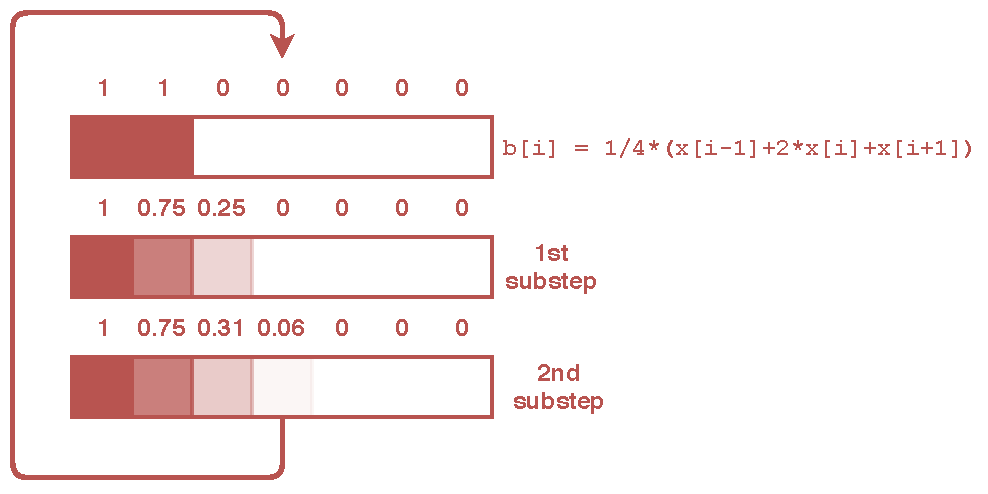
\includegraphics[width=.7\textwidth]{blur_twice_kernel}
  \end{figure}
\end{frame}


\begin{frame}{Hands-on}{Exercise 3 -- 1D blur kernel}
  \begin{itemize}
  \item \shinline{practicals/basics/blur_openacc.\{cpp,f90\}}
  \item Run as: \shinline{srun --reserv=openacc -Cgpu ./blur.openacc [ARRAY\_SIZE]}
    \begin{itemize}
    \item \shinline{ARRAY\_SIZE} is power of 2, default is 20
    \end{itemize}
  \item Offload to GPU the loops of the naive kernel; why is it so slow?
    \pause
    \vfill
  \item Moving data to and from the device is slow ($\approx$7--8\,GB/s per direction)
  \item Avoid unnecessary data movement in the \texttt{nocopies} kernel
    \begin{itemize}
    \item Move the necessary data to GPU early enough and keep it there as long as possible
    \item Update host copies using \lstinlineCpp{\#pragma acc update} directive if needed
    \end{itemize}
  \end{itemize}
\end{frame}


\begin{frame}{Hands-on}{Exercise 4 -- Experiment with the unified memory}
  \begin{itemize}
  \item Remove all the data directives and data clauses
  \item Compile the \texttt{blur\_twice\_naive} kernel with \texttt{-Mcuda=managed}
  \item How does it compare to the manual data management in terms of performance?
  \item Can you explain the performance difference?
  \end{itemize}
\end{frame}


\begin{frame}{Asynchronous execution and wait queues}
  By default, all OpenACC directives are blocking.
  \vspace\baselineskip
  \begin{itemize}
  \item The calling CPU thread must wait for the OpenACC operation (data
    transfer, kernel etc.) to complete
  \item All OpenACC operations are enqueued in a single \emph{activity queue} (CUDA stream)
  \item All items in an activity queue are executed synchronously, but activity queues are independent from each other
  \end{itemize}
\end{frame}

\begin{frame}{Asynchronous execution and wait queues}
  OpenACC allows you to enqueue operations on different activity queues using the \lstinlineCpp{async} clause and wait for them using the \lstinlineCpp{wait} directive/clause.
  \vfill
  \begin{itemize}
  \item \lstinlineCpp{async(<qno>)}: push operations to activity queue \texttt{qno} and continue execution on the host
  \item \lstinlineCpp{wait(<qno>)}: wait for pending operations in activity queue \texttt{qno} to finish before launching next operation on the device
  \item \lstinlineCpp{\#pragma acc wait(<qno>)}: Wait for all events in activity queue \texttt{qno} to finish before continuing execution on the host
    \begin{itemize}
    \item Wait for all queues to finish if used without an argument
    \end{itemize}
  \end{itemize}
\end{frame}

\begin{frame}[fragile]{Asynchronous execution and wait queues}{Example of operations pipelining}
  \begin{Cpplisting}{Operations are executed sequentially}
#pragma acc data ...
for (auto p = 0; p < n; ++p) {
    #pragma acc update device update device(A[p][0:m])
    #pragma acc parallel loop
    for (auto i = 0; i < m; ++i) {
        // work on A[p] array
    }

    #pragma acc update host(A[p][0:m])
}
  \end{Cpplisting}
\end{frame}

\begin{frame}[fragile]{Asynchronous execution and wait queues}{Example of operations pipelining}
  \begin{Cpplisting}{Operations are pipelined}
#pragma acc data ...
for (auto p = 0; p < n; ++p) {
    #pragma acc update device update device(A[p][0:m]) async(p)
    #pragma acc parallel loop async(p)
    for (auto i = 0; i < m; ++i) {
        // work on A[p] array
    }

    #pragma acc update host(A[p][0:m]) async(p)
}
#pragma acc wait
  \end{Cpplisting}
  \vfill
  This concept is useful for overlapping computation and data transfers to the device.
\end{frame}

\begin{frame}{Interoperability with CUDA}
  \large
  \begin{itemize}
  \item Can I use a CUDA pointer inside OpenACC context?
    \vspace\baselineskip
  \item Can I call a CUDA function from OpenACC context?
  \end{itemize}
  \vfill
  Short answer is \emph{yes}.
\end{frame}

\begin{frame}{Interoperability with CUDA}{Use CUDA pointers inside OpenACC context}
  A scenario:
  \begin{itemize}
  \item Have a CUDA code that needs to call a function that uses OpenACC.
  \item This function may accept an array that has been allocated already on the GPU by CUDA.
  \end{itemize}
  \vfill
  The problem?
  \begin{itemize}
  \item OpenACC only knows of pointers that it is managing itself; the \texttt{present} clause won't work. No idea what this pointer is; never seen it before!
  \end{itemize}
\end{frame}

\begin{frame}{Interoperability with CUDA}{Use CUDA pointers inside OpenACC context}
  Solution:
  \vspace\baselineskip
  \begin{itemize}
  \item We need to instruct the OpenACC runtime to trust this pointer and that it is a valid device pointer.
  \item OpenACC runtime will just treat that pointer as known, but it won't check its shape.
  \item Use the \lstinlineCpp{deviceptr(<ptrlist>)} clause with
    \lstinlineCpp{parallel}, \lstinlineCpp{kernels} and \lstinlineCpp{data} directives
  \end{itemize}
\end{frame}

\begin{frame}[fragile]{Interoperability with CUDA}{Use CUDA pointers inside OpenACC context -- Example}
  \begin{lstlisting}[style=CppStyle]
void copy(double *dst, const double *src, size_t n) {
  #pragma acc parallel loop deviceptr(dst, src)
  for (size_t i = 0; i < n; ++i) {
    dst[i] = src[i];
  }
}

int main() {
  double *a, *b;
  cudaMalloc(&a, 1024);
  cudaMalloc(&b, 1024);
  ...
  copy(b, a, 1024);
  return 0;
}
  \end{lstlisting}
\end{frame}

\begin{frame}[fragile]{Interoperability with CUDA}{Call a CUDA function from OpenACC context}
  Scenario:
  \begin{itemize}
  \item My code is in OpenACC, but I need to call an optimized library written in CUDA, which accepts device pointers, e.g., cuBLAS.
  \end{itemize}
  \pause
  Problem:
  \begin{itemize}
  \item I only ``see'' device pointers while in a parallel region, but I want to get a device pointer, while executing on the host.
  \end{itemize}
  \pause
  Solution:
  \begin{itemize}
  \item Use a \lstinlineCpp{host_data} region
    \begin{itemize}
    \item \lstinlineCpp{#pragma acc host_data use_device(<varlist>)}
    \end{itemize}
  \end{itemize}
\end{frame}

\begin{frame}[fragile]{Interoperability with CUDA}{The \texttt{host\_data} directive}
  \begin{itemize}
  \item C/C++: \lstinlineCpp{#pragma acc host_data use_device(<varlist>)}
    \begin{itemize}
    \item In the next block of code the compiler will make available the device address of any variable in \texttt{<varlist>}.
    \end{itemize}
  \item Fortran: \lstinlineFortran{\!\$acc host_data use_device(<varlist>)}
    \begin{itemize}
    \item The compiler will make available the device address of any variable in \texttt{<varlist>} until a matching \lstinlineFortran{\!\$acc end host_data} is found.
    \end{itemize}
  \item Optional clauses:
    \begin{itemize}
    \item \texttt{if(\emph{condition})}: Use the device pointer if \texttt{\emph{condition}} is true.
    \item \texttt{if\_present}: Use the device pointer if variables in \texttt{<varlist>} are present on the device.
    \end{itemize}
  \end{itemize}
  \small\emph{Heads-up: Remember this directive when you will learn about MPI and RDMA next week.}
\end{frame}


%% \begin{frame}{Interoperability with MPI}{The communication data path}
%%   \begin{figure}
%%     \centering
%%     \only<1>{
%%       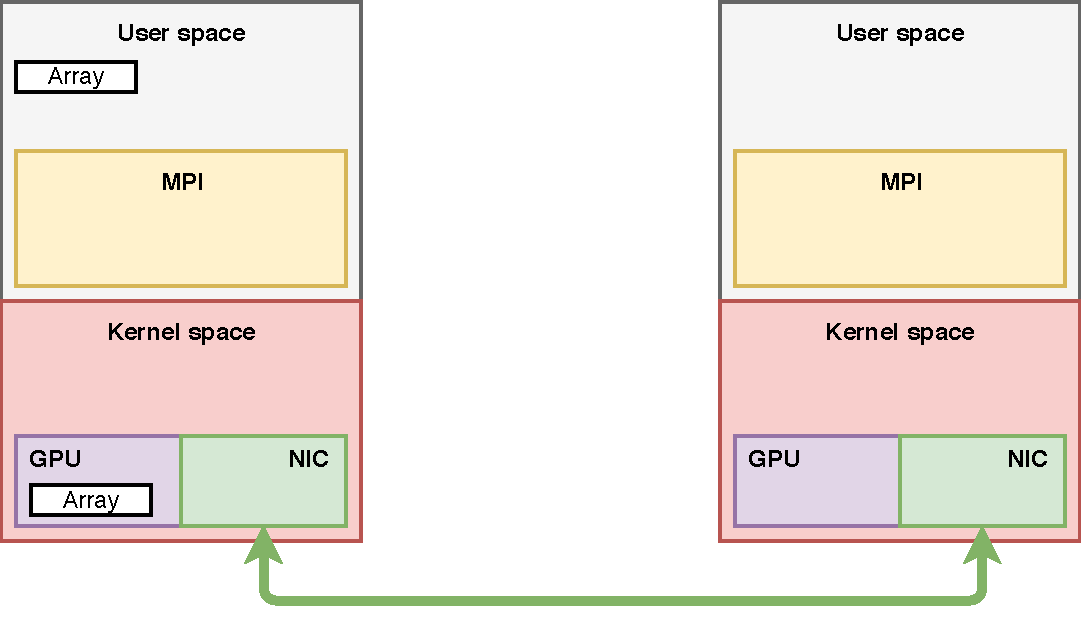
\includegraphics[height=.7\textheight]{rdma_unoptimized_initstate}
%%     }
%%     \only<2>{
%%       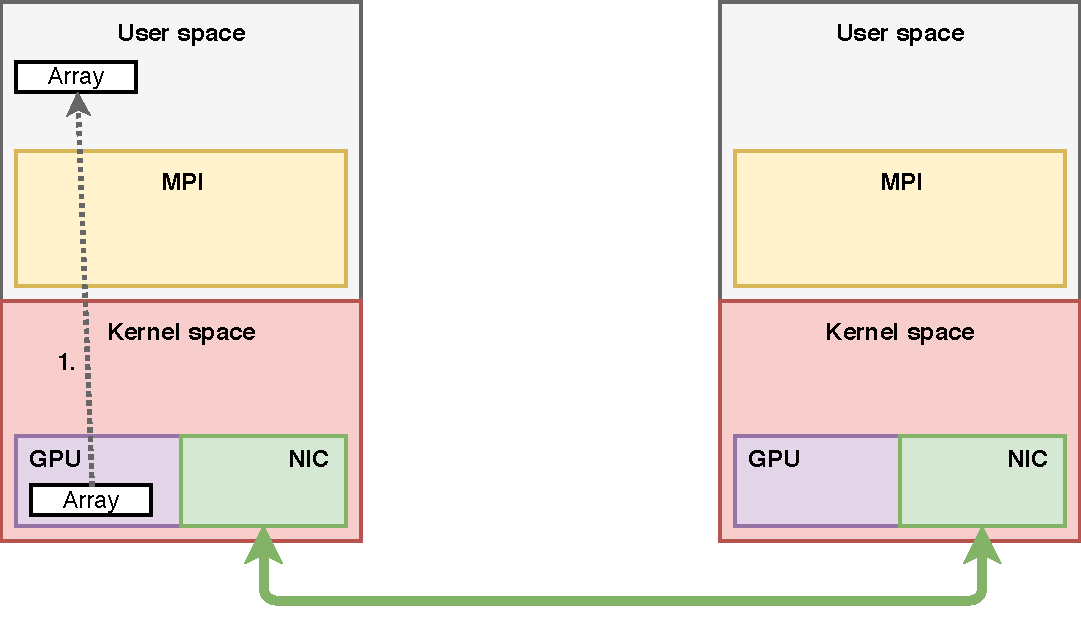
\includegraphics[height=.7\textheight]{rdma_unoptimized_update_host}
%%     }
%%     \only<3>{
%%       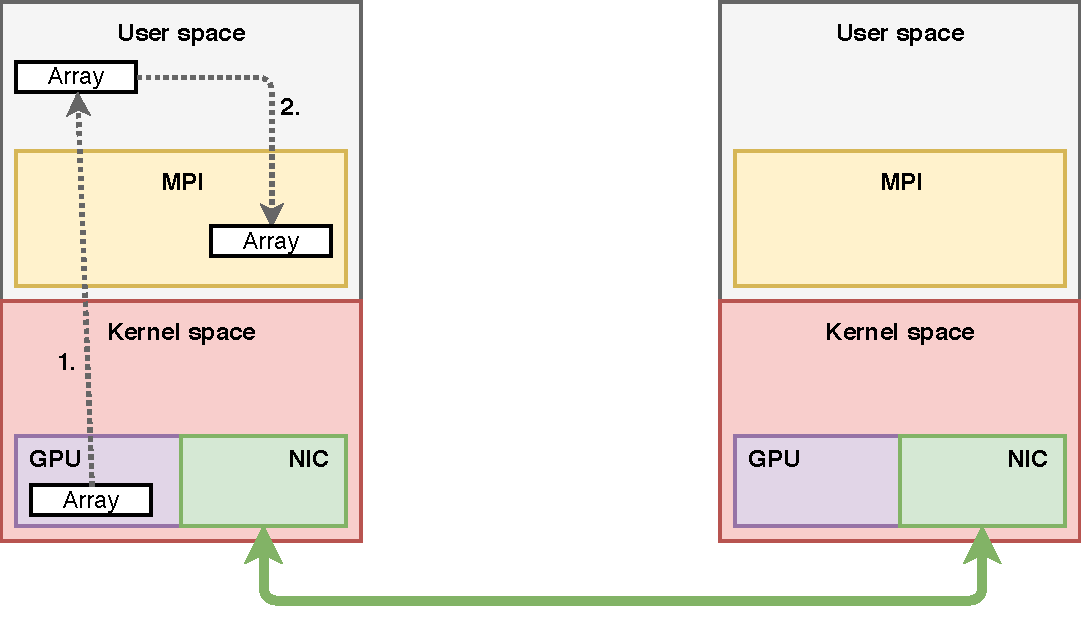
\includegraphics[height=.7\textheight]{rdma_unoptimized_mpi_copy}
%%     }
%%     \only<4>{
%%       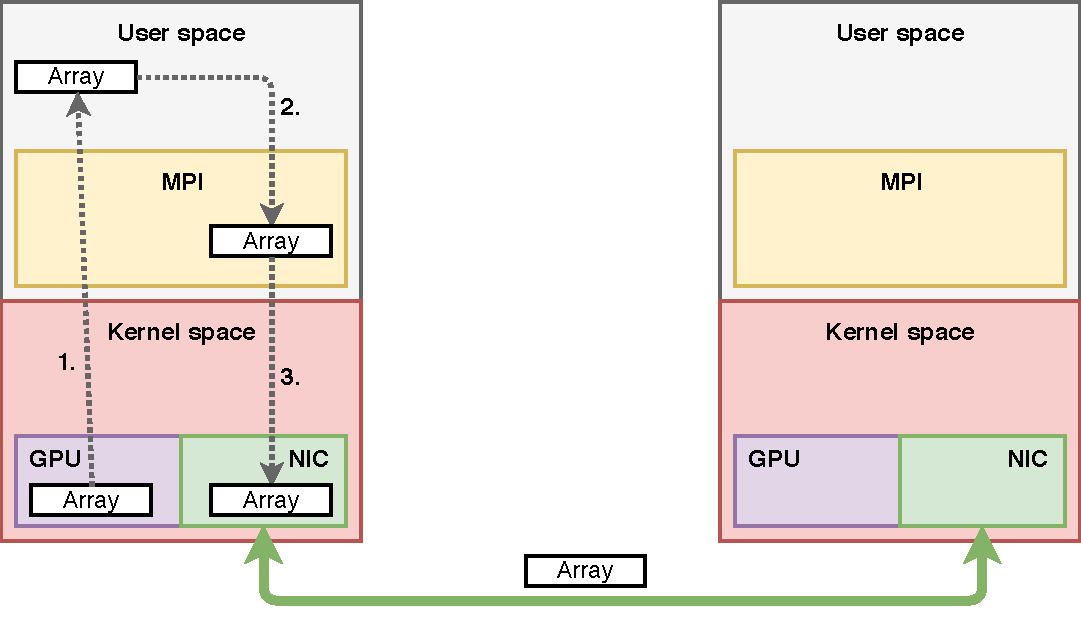
\includegraphics[height=.7\textheight]{rdma_unoptimized_nic_copy}
%%     }
%%     \only<5>{
%%       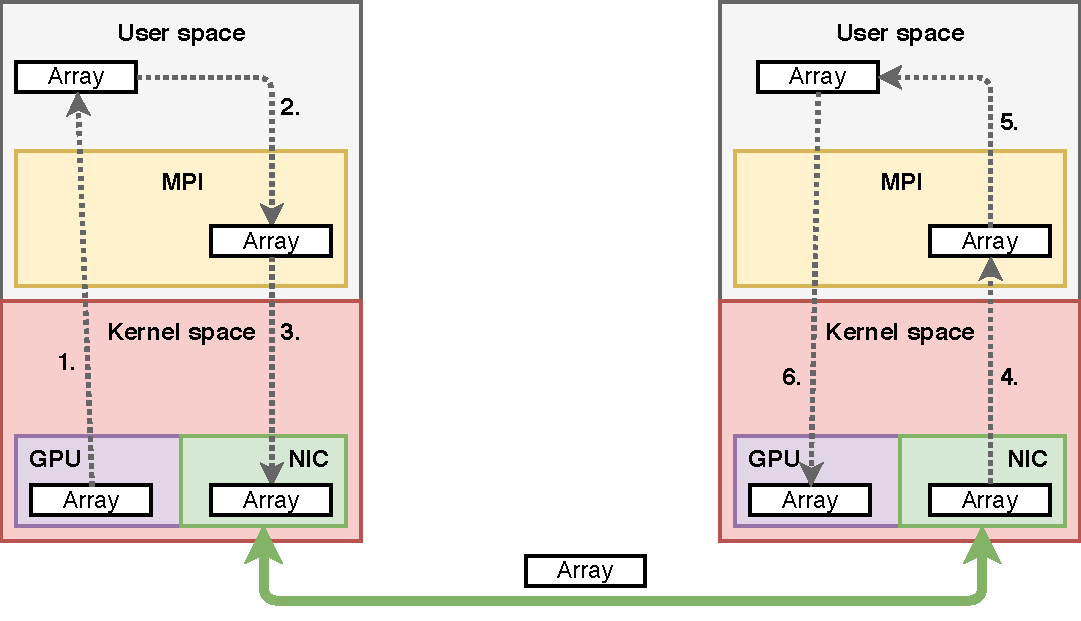
\includegraphics[height=.7\textheight]{rdma_unoptimized_recv}
%%     }
%%   \end{figure}
%% \end{frame}

%% \begin{frame}{Interoperability with MPI}{The communication data path}
%%   \begin{itemize}
%%   \item Aren't there too many copies?
%%   \item This path is not fully unoptimized though! It still bypasses a copy by enabling RDMA between the NICs.
%%   \end{itemize}
%%   \pause
%%   \vfill
%%   Ideally, we would like to avoid all these copies and have the GPU talk directly to the NIC.
%%   \begin{itemize}
%%   \item Answer: GPUDirect
%%   \end{itemize}
%% \end{frame}

%% \begin{frame}{Interoperability with MPI}{The GPUDirect optimized RDMA path}
%%   \begin{figure}
%%     \centering
%%     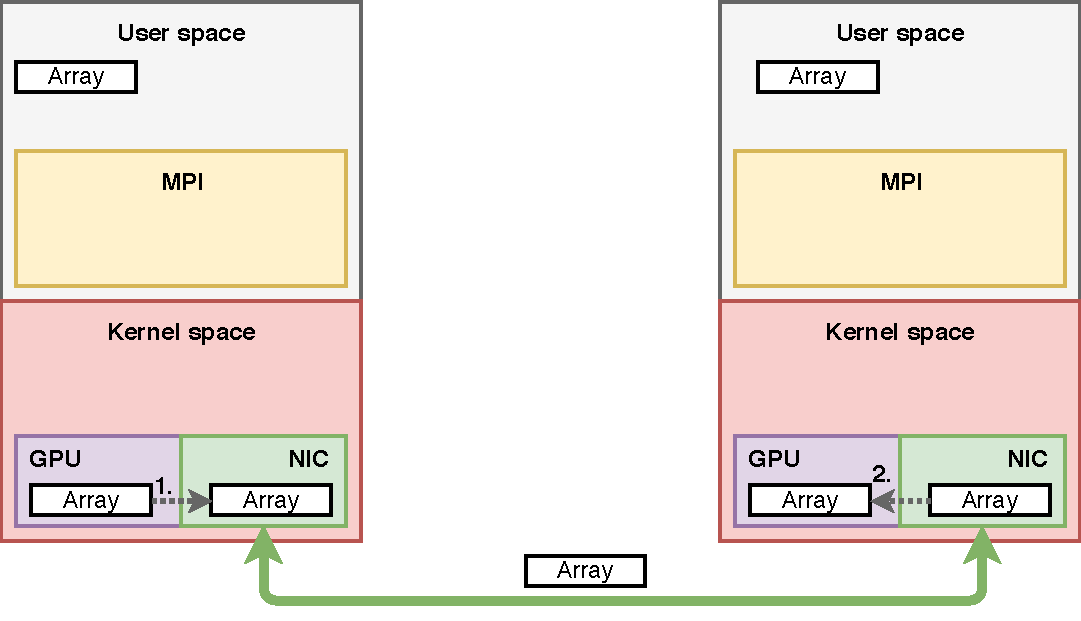
\includegraphics[height=.7\textheight]{rdma_gpudirect}
%%   \end{figure}
%% \end{frame}

%% \begin{frame}{Interoperability with MPI}{How to enable this optimized path with OpenACC}
%%   \begin{itemize}
%%   \item The MPI implementation \emph{must} support it! Cray MPICH implementation does.
%%     \begin{itemize}
%%     \item Enabled by setting \shinline{MPICH_RDMA_ENABLED_CUDA=1}.
%%     \end{itemize}
%%     \vspace\baselineskip
%%   \item If a GPU pointer passed in Send/Recv call, the MPI implementation enables the optimized GPUDirect data path.
%%     \pause
%%     \vspace\baselineskip
%%   \item Wrap the Send/Recv calls using the \lstinlineCpp{host_data} directive to get the OpenACC device pointers.
%%   \end{itemize}
%% \end{frame}

\begin{frame}[fragile]{Hands-on}{Exercise 5 -- Calling cuBLAS methods}
  Source code:
  \begin{itemize}
  \item \shinline{practicals/gemm/gemm.cpp}
  \item Run as: \shinline{srun --reserv=openacc -Cgpu ./axpy.openacc [ARRAY\_SIZE]}
    \begin{itemize}
    \item \shinline{ARRAY\_SIZE} is power of 2, default is 16
    \end{itemize}
  \end{itemize}
  \vfill
  Steps:
  \begin{enumerate}
  \item Compile with `\shinline{make CPPFLAGS=}' to get also the naive implementation $\rightarrow$ too slow!
  \item Offload the GEMM method to the GPU using OpenACC
  \item Make use of cuBLAS GEMM through OpenACC
  \item When does it start to pay of using cuBLAS?
  \end{enumerate}
\end{frame}

\begin{frame}[fragile]{Hands-on}{Exercise 6.1 -- 2D diffusion example}
  Source code:
  \begin{itemize}
  \item \shinline{diffusion2d\_omp.\{cpp,f90\}}: our baseline code
    \begin{itemize}
    \item Single node OpenMP version for the CPU
    \end{itemize}
  \item \shinline{diffusion2d\_openacc.\{cpp,f90\}}
    \begin{itemize}
    \item Single node OpenACC version
      \item Run as: \shinline{srun --reserv=openacc -Cgpu ./diffusion2d.openacc [ARRAY\_SIZE]}
        \begin{itemize}
        \item \shinline{ARRAY\_SIZE} is power of 2, default is 16
        \end{itemize}
      \item Fill in the parts where \lstinlineCpp{OPENACC_DATA} is defined.
    \end{itemize}
  \end{itemize}
\end{frame}

\begin{frame}[fragile]{Hands-on}{Exercise 6.2 -- 2D diffusion example using CUDA data management}
  Source code:
  \begin{itemize}
  \item \shinline{diffusion2d\_openacc.\{cpp,f90\}}
    \begin{itemize}
    \item Single node OpenACC version
      \item Run as: \shinline{srun --reserv=openacc -Cgpu ./diffusion2d.openacc.cuda [ARRAY\_SIZE]}
        \begin{itemize}
        \item \shinline{ARRAY\_SIZE} is power of 2, default is 16
        \end{itemize}
      \item Fill in the parts where \lstinlineCpp{OPENACC_DATA} is defined.
    \end{itemize}
  \end{itemize}
\end{frame}

\begin{frame}[fragile]{Hands-on}{Exercise 6.3 -- 2D diffusion example using MPI}
  Source code:
  \begin{itemize}
  \item \shinline{diffusion2d\_openacc_mpi.\{cpp,f90\}}
    \begin{itemize}
      \item Run as: \shinline{srun --reserv=openacc -Cgpu ./diffusion2d.openacc.cuda [ARRAY\_SIZE]}
        \begin{itemize}
        \item \shinline{ARRAY\_SIZE} is power of 2, default is 16
        \end{itemize}
      \item Fill in the parts where \lstinlineCpp{OPENACC_DATA} is defined.
    \end{itemize}
  \end{itemize}
\end{frame}

\begin{frame}[fragile]{Deep Copy}{The concept}
  \vspace{.5\baselineskip}
  \begin{Cpplisting}{True deep copy (ideal)}
struct foo {
    int *arr;
    size_t len;
};
// ...
for (auto i = 0; i < 3; ++i) {
    f[i].len = 10;
    f[i].arr = new int[f[i].len];
}

#pragma acc enter data copyin(f[0:3])
  \end{Cpplisting}
  \begin{itemize}
  \item Where will \lstinlineCpp{f[i].arr} refer to?
    \onslide<2->{$\rightarrow$ They will be host pointers!}
  \item<2-> Ideally, we would like everything to be magically copied.
    \begin{itemize}
    \item Not so easy, especially for C/C++.
    \end{itemize}
  \end{itemize}

\end{frame}

\begin{frame}[fragile]{Deep Copy}{The manual solution -- OpenACC 2.6}
  \begin{Cpplisting}{Manual deep copy (top-down approach)}
#pragma acc enter data copyin(f[0:3])
for (auto i = 0; i < 3; ++i) {
    #pragma acc enter data copyin(f[i].arr[0:f[i].len])
}
// do stuff on the device
for (auto i = 0; i < 3; ++i) {
    #pragma acc exit data copyout(f[i].arr[0:f[i].len])
}
#pragma acc exit data copyout(f[0:3])
  \end{Cpplisting}
  \begin{itemize}
  \item The runtime will attach the \lstinlineCpp{f[i].arr} pointer to the device copy of the data.
  \item This happens implicitly if the \lstinlineCpp{f[i].arr} pointer is present on the device.
  \end{itemize}
\end{frame}

\begin{frame}[fragile]{Deep Copy}{The manual solution -- OpenACC 2.6}
  \vspace{.5\baselineskip}
  \begin{Cpplisting}{Manual deep copy (bottom-up approach)}
for (auto i = 0; i < 3; ++i) {
    #pragma acc enter data copyin(f[i].arr[0:f[i].len])
}

#pragma acc enter data copyin(f[0:3])
for (auto i = 0; i < 3; ++i) {
    acc_attach((void **) &f[i].arr);
}
// do stuff on the device
  \end{Cpplisting}
  \begin{itemize}
  \item At the time when \lstinlineCpp{f[i].arr} is copied to the device, the pointer is not already present on the device.
  \item If we copy the \lstinlineCpp{struct} later, we need to manually attach the pointer to the device copy of the data.
  \end{itemize}
\end{frame}

%% \begin{frame}[fragile]{Outlook}
%%   OpenACC 2.6 is due end of the year
%%   \begin{itemize}
%%   \item Manual deep copy
%%   \item Standardize behavior of Fortran optional arguments
%%   \item Fortran bindings for all API routines
%%   \item \lstinlineCpp{acc serial} directive
%%   \item Device query routines
%%   \item Improvements in error handling
%%   \end{itemize}
%%   OpenACC 3.0
%%   \begin{itemize}
%%   \item Not scheduled yet
%%   \item The big feature should be the true deep copy
%%   \end{itemize}
%% \end{frame}


\begin{frame}{OpenACC vs.\ OpenMP}
  \begin{itemize}
    \vfill
  \item OpenMP 4.0 introduced directives for offloading computation to accelerators
    \vfill
  \item Similar concepts to OpenACC but OpenMP is a more prescriptive standard
    \vfill
  \item There is no OpenMP-OpenACC merger envisioned right now
    \vfill
  \item Compiler support for GPU targets
    \begin{itemize}
    \item Cray
    \item IBM XL
    \item GCC (needs to be compiled specially)
    \item Clang (under development)
    \end{itemize}
  \end{itemize}
\end{frame}

\begin{frame}{OpenACC and compiler support}
  \begin{itemize}
  \item PGI
    \begin{itemize}
    \item Latest spec support; drives the OpenACC development
    \item Twice per year a community release
    \end{itemize}
  \item Cray
    \begin{itemize}
    \item Support up to OpenACC 2.0; no new features or later spec support
    \item Bug fixes and support for the current implementation only
    \end{itemize}
  \item GCC
    \begin{itemize}
    \item Support of OpenACC 2.0a from GCC 5.1 onward
    \item Support of OpenACC 2.5 in development branch
    \end{itemize}
  \end{itemize}
\end{frame}

\begin{frame}{More information and events}
  \begin{itemize}
  \item \url{http://www.openacc.org}
    \begin{itemize}
    \item Specification and related documents
    \item Tutorials
    \item Events
    \end{itemize}
    \vfill
  \item GPU Hackathons
    \begin{itemize}
    \item One week of intensive development for porting your code to the GPUs
    \item 3 developers + 2 mentors per team
    \item 7 events scheduled for 2018 (Australia, Europe, United States)
    \item Find the one that fits you and apply!
    \end{itemize}
  \end{itemize}
\end{frame}

%% \part{Porting the miniapp to GPUs using OpenACC}

%% \begin{frame}[fragile]{General info}
%%   \begin{itemize}
%%   \item Fortran 90 version
%%     \begin{itemize}
%%     \item \lstinlineCpp{miniapp/openacc/fortran/}
%%     \end{itemize}
%%   \item C++11 version
%%     \begin{itemize}
%%     \item \lstinlineCpp{miniapp/openacc/cxx/}
%%     \item Compile with PGI 17.4
%%       \begin{itemize}
%%         \item\shinline{module switch PrgEnv-cray PrgEnv-pgi}
%%         \item\shinline{source <ss-prefix>/scripts/setup.sh}
%%         \item\shinline{module switch pgi/16.9.0 pgi/17.4}
%%       \end{itemize}
%%     \end{itemize}
%%   \item Interesting files
%%     \begin{itemize}
%%     \item\shinline{main.\{cpp,f90\}}: the solver
%%     \item\shinline{data.\{h,f90\}}: domain types
%%     \item\shinline{linalg.\{cpp,f90\}}: linear algebra kernels
%%     \item\shinline{operators.\{cpp,f90\}}: the diffusion kernel
%%     \end{itemize}
%%   \end{itemize}
%% \end{frame}

%% \begin{frame}{Notes for the C++ version}
%%   \begin{itemize}
%%   \item There are two C++-isms that complicate things:
%%     \begin{enumerate}
%%     \item Domain data is encapsulated inside the \lstinlineCpp{Field} class
%%       \begin{itemize}
%%       \item Allocated and initialised inside the constructor
%%       \item Deallocated inside the destructor
%%       \end{itemize}
%%     \item Operators for accessing the domain data
%%     \end{enumerate}
%%     \vfill
%%   \item OpenACC provides the \lstinlineCpp{enter data} and \lstinlineCpp{exit
%%     data} directives for unscoped data management
%%   \item Operators are just another kind of functions
%%     \begin{itemize}
%%     \item \lstinlineCpp{acc routine} directive is just for that
%%     \end{itemize}
%%   \item Remember to copy the object itself (\lstinlineCpp{this} pointer)
%%   \end{itemize}
%% \end{frame}

\end{document}
